\documentclass[11pt]{article}
% \usepackage{times}
\usepackage{booktabs}
\usepackage{palatino}
\usepackage{fontspec}
\usepackage[colorlinks,linkcolor=blue]{hyperref}
\usepackage{amsmath}
\usepackage{enumitem}
\usepackage{algorithm}
\usepackage{algorithmicx}
\usepackage{algpseudocode}
\usepackage{graphicx}
\usepackage{multirow}
\setmainfont{Times New Roman}
\renewcommand{\algorithmicrequire}{\textbf{input:}}
\renewcommand{\algorithmicensure}{\textbf{output:}}

\renewcommand{\baselinestretch}{1.2}
\setlength{\topmargin}{-0.5in}
\setlength{\textwidth}{6.5in}
\setlength{\oddsidemargin}{0.0in}
\setlength{\textheight}{9.1in}

\usepackage[super,square,numbers,sort&compress]{natbib}

\usepackage[utf8]{inputenc}

\usepackage{listings}
\usepackage{color}

\definecolor{codegreen}{rgb}{0,0.6,0}
\definecolor{codegray}{rgb}{0.5,0.5,0.5}
\definecolor{codepurple}{rgb}{0.58,0,0.82}
\definecolor{backcolour}{rgb}{0.95,0.95,0.92}

\lstdefinestyle{mystyle}{
	backgroundcolor=\color{backcolour},   
	commentstyle=\color{codegreen},
	keywordstyle=\color{magenta},
	numberstyle=\tiny\color{codegray},
	stringstyle=\color{codepurple},
	basicstyle=\footnotesize,
	breakatwhitespace=false,         
	breaklines=true,                 
	captionpos=b,                    
	keepspaces=true,                 
	numbers=left,                    
	numbersep=5pt,                  
	showspaces=false,                
	showstringspaces=false,
	showtabs=false,                  
	tabsize=2
}

\lstset{style=mystyle}

\usepackage{hyperref}
\makeatletter
\def\UrlAlphabet{%
	\do\a\do\b\do\c\do\d\do\e\do\f\do\g\do\h\do\i\do\j%
	\do\k\do\l\do\m\do\n\do\o\do\p\do\q\do\r\do\s\do\t%
	\do\u\do\v\do\w\do\x\do\y\do\z\do\A\do\B\do\C\do\D%
	\do\E\do\F\do\G\do\H\do\I\do\J\do\K\do\L\do\M\do\N%
	\do\O\do\P\do\Q\do\R\do\S\do\T\do\U\do\V\do\W\do\X%
	\do\Y\do\Z}
\def\UrlDigits{\do\1\do\2\do\3\do\4\do\5\do\6\do\7\do\8\do\9\do\0}
\g@addto@macro{\UrlBreaks}{\UrlOrds}
\g@addto@macro{\UrlBreaks}{\UrlAlphabet}
\g@addto@macro{\UrlBreaks}{\UrlDigits}
\makeatother

\newlength{\pagewidth}
\setlength{\pagewidth}{6.5in}
\pagestyle{empty}

\def\pp{\par\noindent}

\special{papersize=8.5in,11in}
\title{\bf CSE 566 -- 
	Virtual Reality Spring  2019 \\
	Assignment 1: Basic VR - Report \\
}
%\date{December 7, 2018}
\author{Jinghuan Shang -- ID\# 112076155}
\begin{document}
	\maketitle
	\section{Important Links}
	Unity Project File: \url{https://drive.google.com/open?id=1gloup2dACtpGdaUvJmRWZ2B5B2CzyjKQ}\\
	Video: \url{https://drive.google.com/open?id=1jxV9XgUSXkxueC8cOdws_wP6-BcgU2Z6}\\
	\section{Environment Set Up}
	Software used:
	\begin{itemize}
		\item Unity: 2017.4.21f1
		\item Google VR SDK for Unity v1.190.1\cite{googlevrsdk}
	\end{itemize}
	Hardware used: 
	\begin{itemize}
		\item VR Headset: VR SHINECON 3D VR Glasses
		\item Mobile Phone: HUAWEI P10 Plus with Android 8.0
		\item Controller: VR SHINECON Glass Remote Control
	\end{itemize}
	
	\section{Directory Hierarchy}
	Only important files are mentioned.
	\begin{lstlisting}
	VRLab1\-----------------------------Unity project directory
		Assets\---------------------------Assets used in the project
			lab1_first_trail.unity----------Main scene file
			*.cs----------------------------C# script files
			[other directories]\------------Imported assets files\end{lstlisting}
	
	
	\section{Extra Features}
	\subsection{Car Motion}
	The car in the scene will slowly move along the road around the building when the character(camera) teleports into the car. It can correctly turn directions if the current road ends.
	\subsection{Extra View in the Building}
	My building is designed and implement by myself with several 3d objects. Besides the basic view on the first floor, I set another place that the camera can teleport to on the second floor. Just press the button of teleporting into the building again if the current location is on the first floor. The scene on the second floor is an imitation from one of my favorite animation ``Neon Genesis Evangelion''.
	
	\section{Implementation}
	\subsection{House}
	The house, or say the building, is implemented by myself py several 3D objects. Due to not able to create complex 3D polygons for now, I just use many 3D cuboids. The material of the walls on the first floor is glass, which is the same as the car\cite{carassets}.
	
	As for the walls on the second floor, I place my customize texts on it. The texts are actually picture resources serve as textures. The picture is designed manually by myself using a picture editor.
	
	The lamp is from the asset \cite{japanlampassets}. I add an extra cylinder rod beneath it to raise it up.
	The lights in the house and the lamp are controlled by the sunlight. If the intensity of the sunlight is less than $0.5$, lights will be turned on.The road is from the Kajaman's Road - Free\cite{kajamansroadsassets}.
	
	\begin{figure}[htbp]
		\centering
		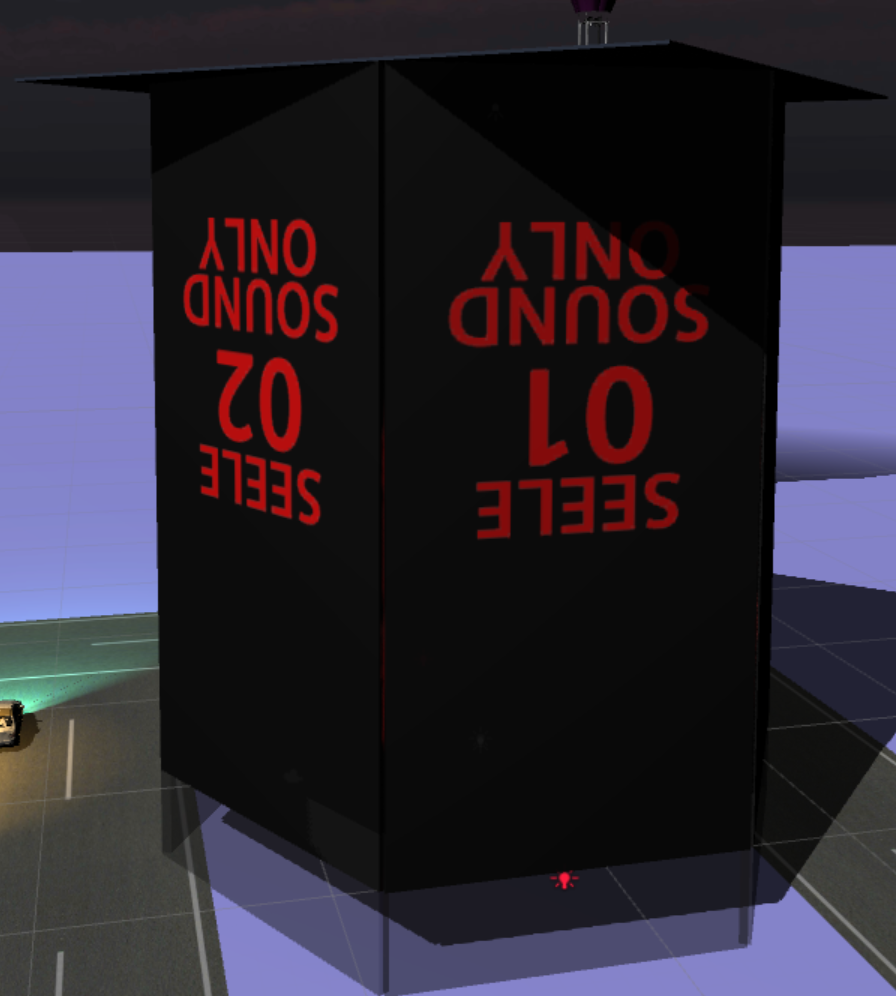
\includegraphics[width=.45\textwidth]{fig/building.png}
		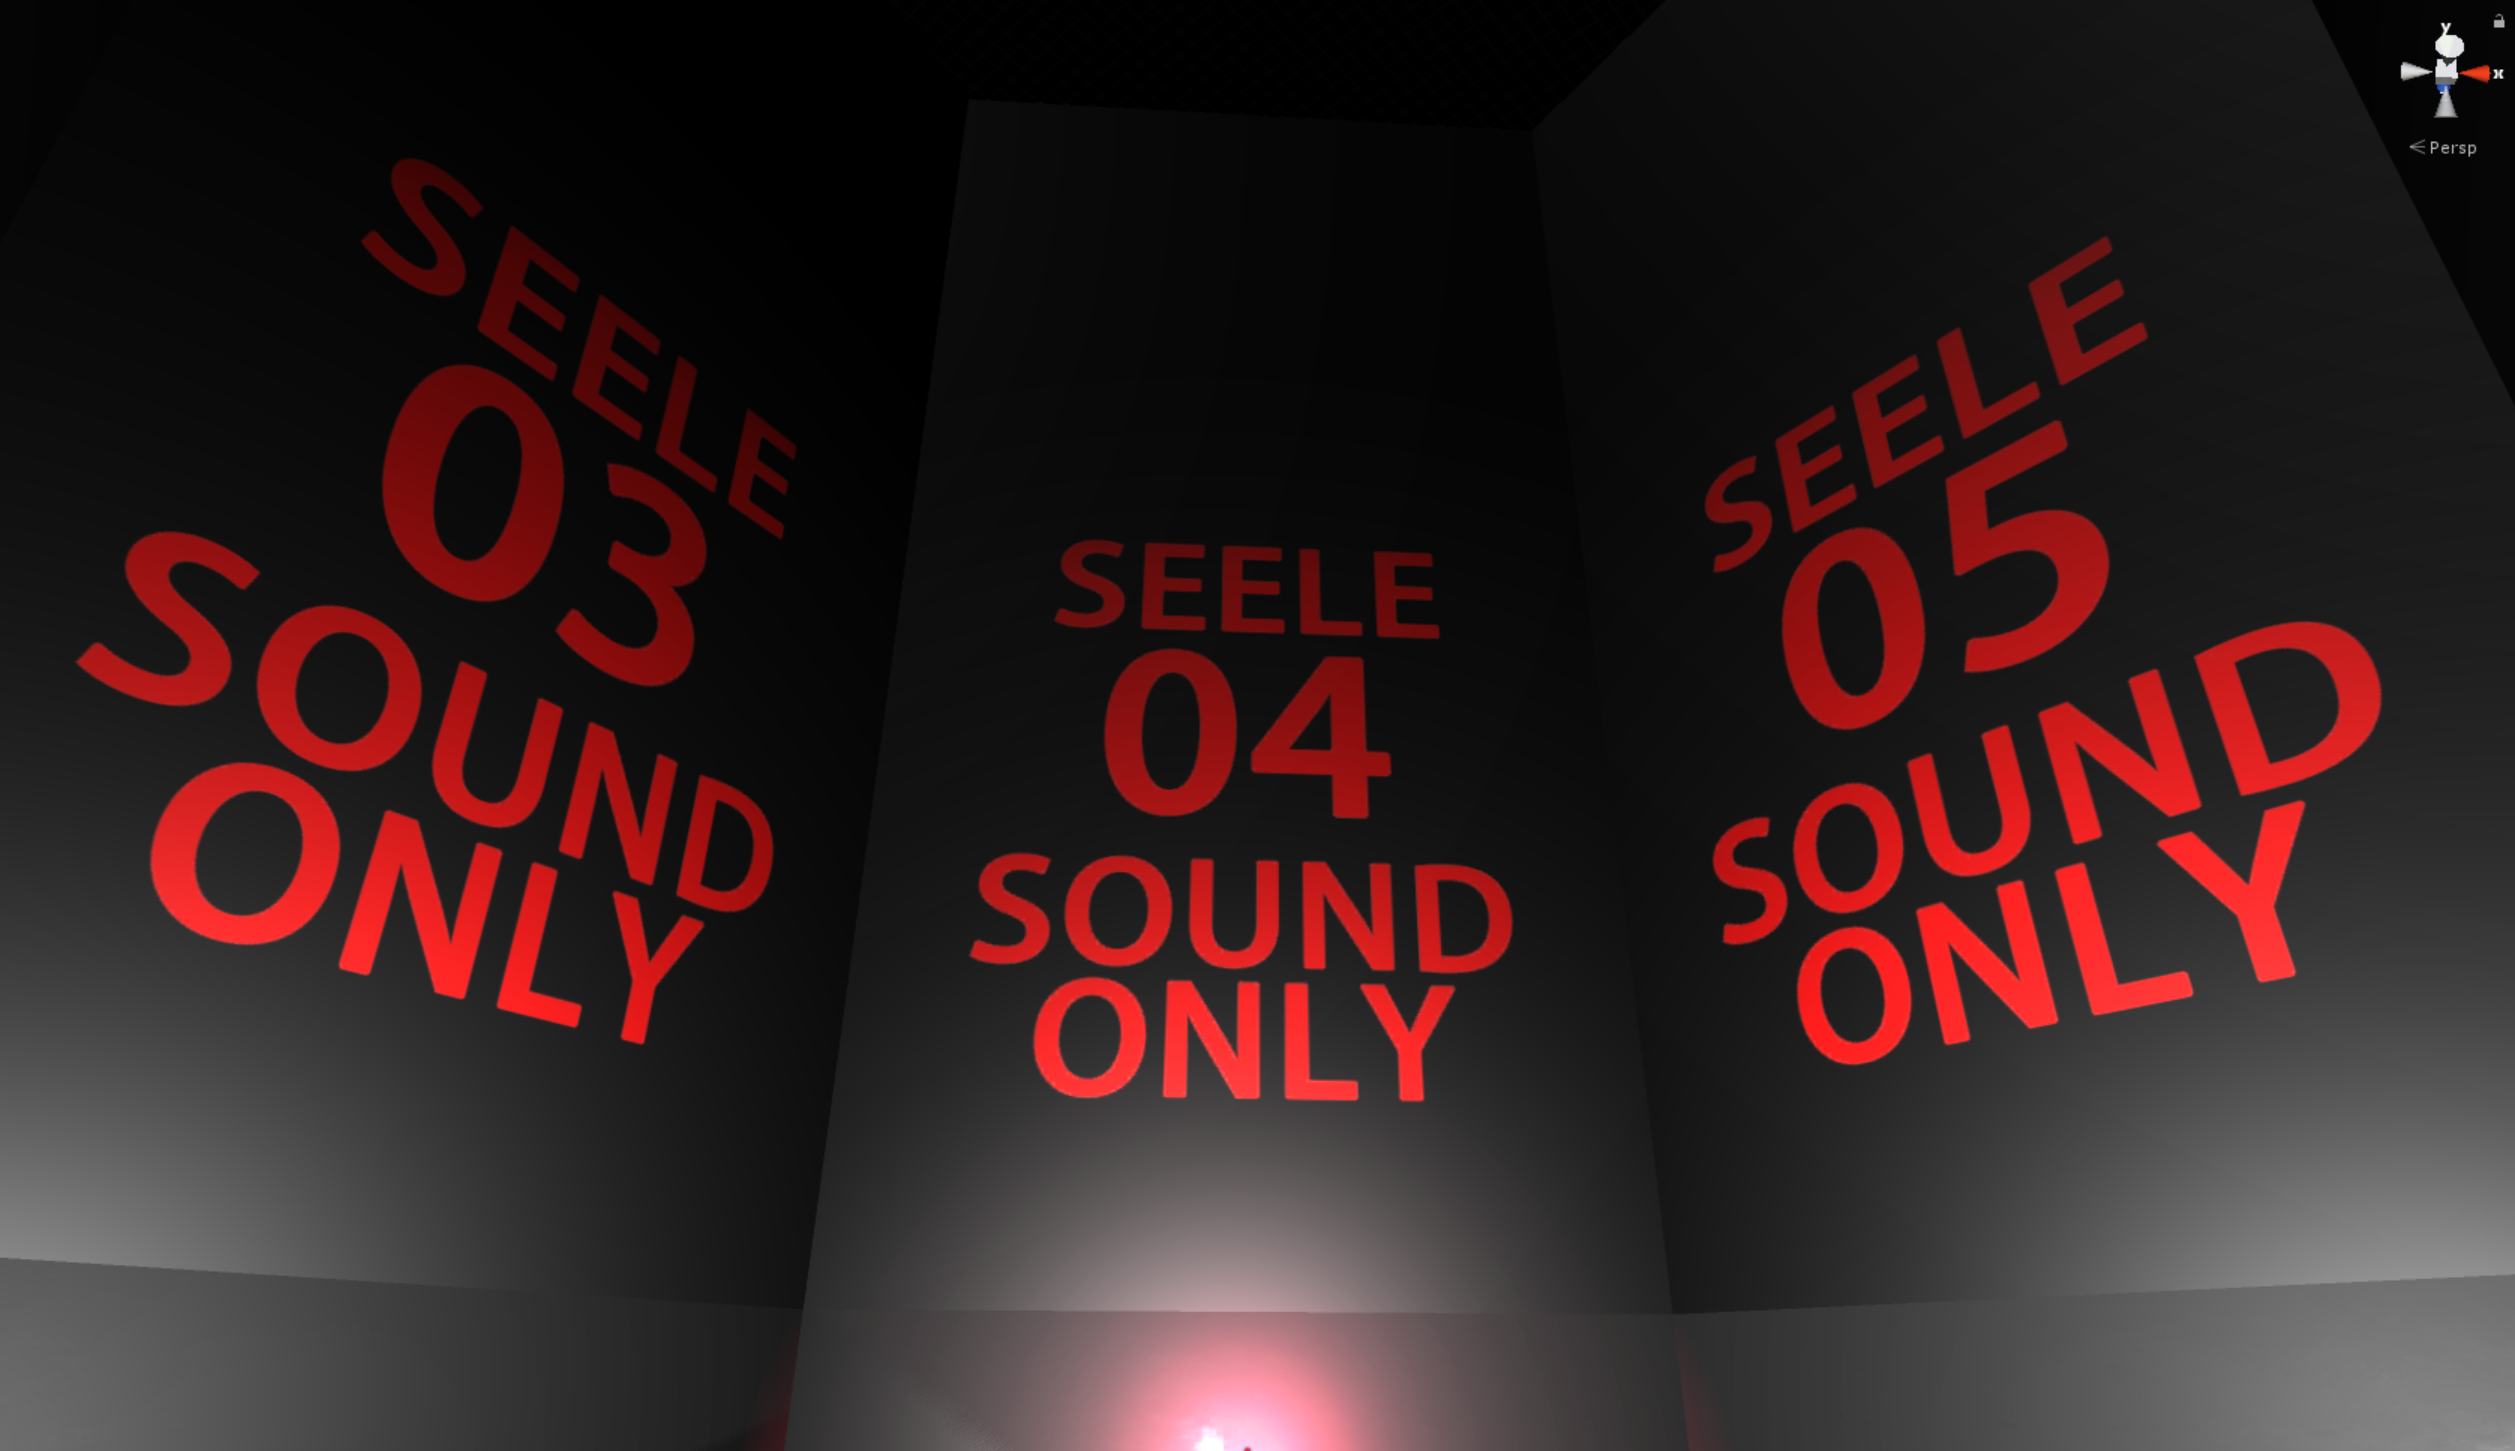
\includegraphics[width=.45\textwidth]{fig/coloregg.png}
		\caption{House and its second floor}
	\end{figure}
	
	
	\subsection{Airplane}
	The airplane (including model, texture and material) is from the asset store\cite{planeassets}.
	The plane can do all the Quaternion rotations. It will go back to its original place when the journey is finished. I control this by recording the original coordinates and remaining time in this round of motion. When time runs out, the plane will be moved to its original place and reset the timer(a float type variable).
	
	The following are Quaternion rotations around $X$, $Y$, and $Z$ axis respectively.
	\begin{lstlisting}
	transform.Rotate(Vector3.right, turnSpeed * Time.deltaTime);
	transform.Rotate(Vector3.up, turnSpeed * Time.deltaTime);
	transform.Rotate(Vector3.forward, turnSpeed * Time.deltaTime);\end{lstlisting}
	
	\begin{figure}[htbp]
		\centering
		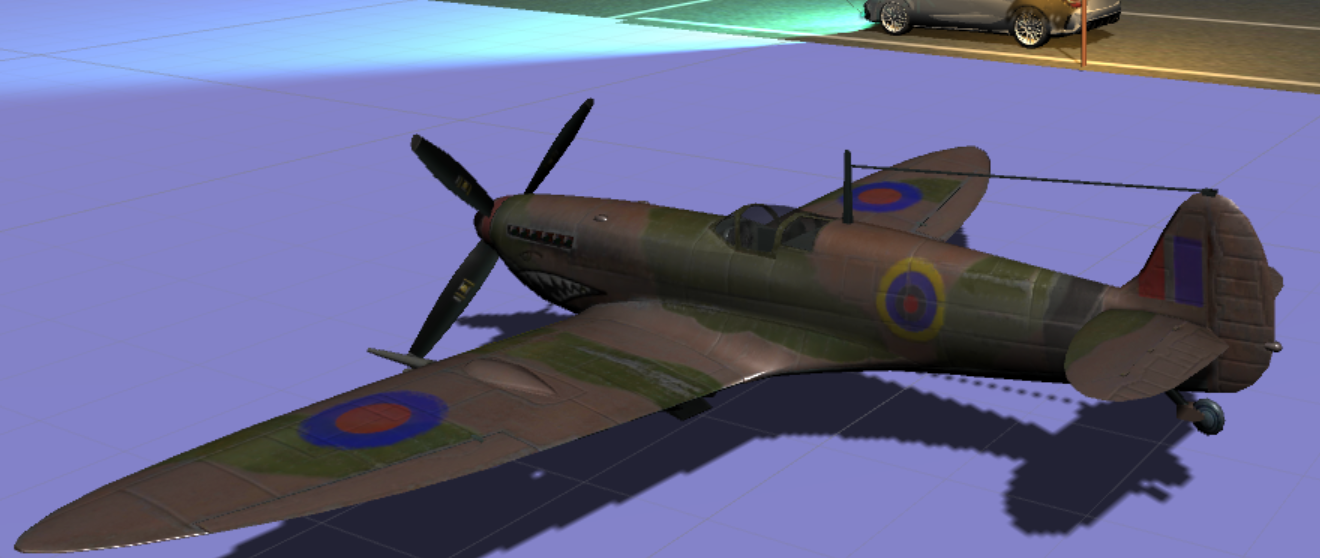
\includegraphics[width=.90\textwidth]{fig/plane.png}
		\caption{Airplane}
	\end{figure}
	
	\subsection{Car}
	The car (including model, texture and material) is from the asset store\cite{carassets}.
	
	The camera position in the car is set by applying a small offset based on the coordinate of the car. When car is moving, Player component gets the position of the car and makes a synced motion by applying same translation vectors to the Player and the car.
	
	The four segments of car motion is maintained by a variable tracking its moving direction and a switch statement. In the switch statement, car is applied rotation translation properly when it will exceeds the current segment of road. The four coordinates indicating the boundaries in the direction of car motion is used to check these switch cases.
	\begin{figure}[htbp]
		\centering
		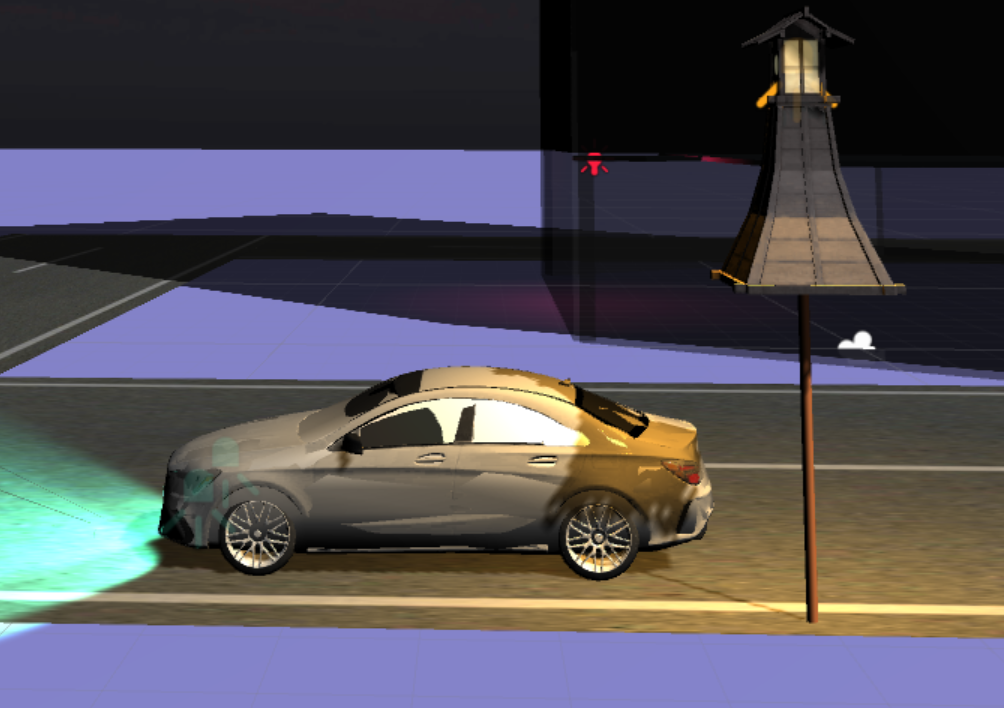
\includegraphics[width=.45\textwidth]{fig/carlamp.png}
		\caption{Car and Lamp}
	\end{figure}
	
	\subsection{Hot Air Balloon}
	The hot air balloon (model and color design) is from the asset store\cite{hotairballoonassets}.
	
	The hot air balloon's trajectory is similar to the car, where this only contains 3 segments of motion. The middle part, where the balloon is simultaneously moving forward and upward, is implemented by apply a translation vector with positive values on both $X$ and $Y$ axes.
	
	\begin{figure}[htbp]
		\centering
		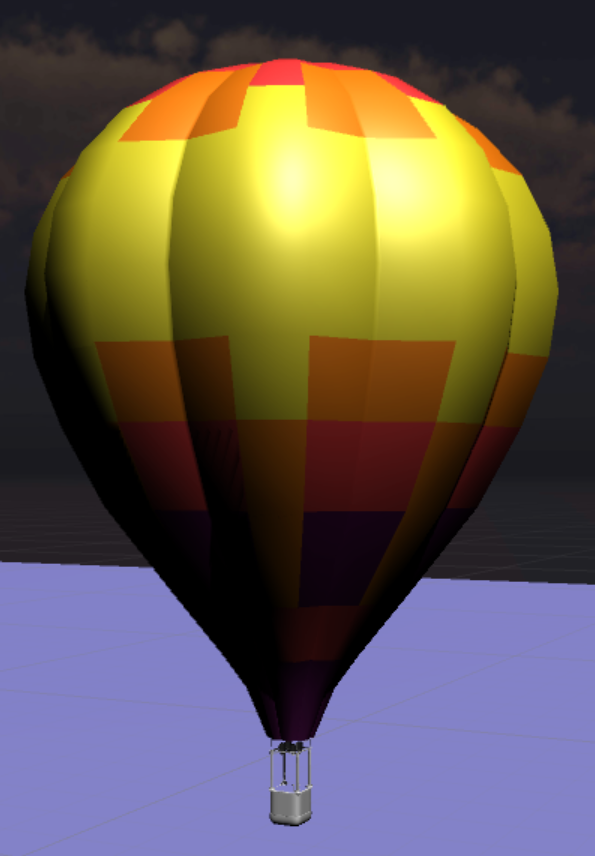
\includegraphics[width=.90\textwidth]{fig/hab.png}
		\caption{Hot Air Balloon}
	\end{figure}
	
	\subsection{Day and Night}
	Day and night changing is implemented by modifying the intensity and the rotation angle of the directional light. The intensity of the `Sun' is designed by equation
	\begin{equation*}
		L(t) = 
		\left\{
			\begin{array}{lr}
				\frac{1-0.005}{150}t + 0.005, & t\in[0, 150)\\
				1, &t\in[150, 300)\\
				1 - \frac{1-0.005}{150}(t-300), & t\in[300, 450)\\
				0.005, & t\in[450, 600)
			\end{array}
		\right.
	\end{equation*}
	where $t$ is cycling between $[0, 600]$, corresponding to 10 minutes in real world. $t\in[150, 450)$ is day and $t\in[0, 150) \cup [450, 600)$ is night.
	The rotation of the ``Sun'' $R_{Sun}(t)$ is in uniform speed. If represented in Euler angle, it starts from $(0, 0, \gamma)$ to $(180, 180, \gamma)$, where $\gamma$ is an arbitrary angle, implemented by 
	\begin{lstlisting}
	transform.Rotate(Vector3.up * angularSpeed * Time.deltaTime * 10 + Vector3.right * angularSpeed * Time.deltaTime * 10);\end{lstlisting}
	This rotation simulates the sunlight changing during the day. 
	When $t>600$, $R_{Sun}(t)$ is reset to $(0, 0, \gamma)$
	
	The ``Moon'' is stationary in the sky with no rotations. It only has $\frac{1}{2}$ brightness of the Sun. When the Sun's intensity is less than a threshold ($0.3$ in my project), the moon's intensity will gradually go up. Their sum will be exactly $0.3$ in case of sudden flash when the moon is ``lighted''. During the day, the Moon's intensity is $0$.
	
	There is another important component called ``Skybox'' in the scene. It simulates the sky above our heads. The Skybox has a parameter ``Exposure'' can be explained as how bright it be in our camera. So when turns to the night, it will also be darker. The value of Exposure is always equals to the sum of the intensities of the Moon and the Sun.
	
	\subsection{Interaction and Camera}
	In my project, I use the Player component in Google VR SDK for Unity\cite{googlevrsdk} to develop my camera and changing of views driven by gyroscope inside the phone.
	
	As for interaction, I utilize 4 keys on the joystick, \textbf{A}, \textbf{B}, \textbf{Y}, and \textbf{X}. The receive is implemented by codes like
	\begin{lstlisting}
	Input.GetKeyDown(KeyCode.Joystick1Button0)\end{lstlisting}
	Interactions are described in the following list.
	\begin{itemize}
		\item[\textbf{A}] Teleport into the building. Press \textbf{A} when in the building again to teleport to the second floor.
		\item[\textbf{B}] Teleport into the car. The car will start its motion along the road, carrying the camera.
		\item[\textbf{Y}] Teleport into the bracket of the hot air balloon. The camera will also follow the motion of hot air balloon.
		\item[\textbf{X}] Teleport back to the initial point where the game starts.
	\end{itemize}
	In order to easy testing, I also bind them with corresponding characters on the keyboard.
	I set a variable to track the current mode. For example, $1$ and $5$ are for in the building, and $2$ for in the car. The variable will help me decide whether and how to update the position of the camera under different modes.
	
	\section{Acknowledgment}
	I would like to thank Xueying Bai and Ying Lu for discussions during this assignment. I also appreciate all the authors of free assets available in the Unity Asset Store.
	%\section{Findings and Results}
	%	Results are shown right in the figures, next to the figure.
	%	\begin{figure}[htbp]
	%		\centering
	%		\includegraphics[width=.90\textwidth]{fig/reselbow.png}
	%		\caption{Elbow Plot}
	%	\end{figure}
	%	\begin{figure}[htbp]
	%		\centering
	%		\includegraphics[width=.90\textwidth]{fig/resscree.png}
	%		\caption{Scree Plot}
	%	\end{figure}
	\bibliography{lab1}
	\bibliographystyle{IEEEtran}
\end{document}


